\documentclass[preprint,12pt,aps,pra,showkeys,amsmath,amssymb,superscriptaddress,floatfix]{revtex4-2}
\usepackage[T1]{fontenc}
\usepackage[utf8]{inputenc}
\usepackage{amsmath,amssymb,amsthm,mathtools,mathrsfs}
\usepackage{microtype,booktabs,enumitem}
\usepackage{xcolor,tikz,etoolbox}
\usepackage[skins,breakable]{tcolorbox}
\usepackage{needspace}
% Keep diagram geometry independent of REVTeX preprint body spacing.
\AtBeginEnvironment{tikzpicture}{\linespread{1}\selectfont}
\usetikzlibrary{arrows.meta,positioning,calc,fit,decorations.pathreplacing}
\usepackage{graphicx}
\usepackage{hyperref}

\definecolor{MMBlue}{RGB}{0,82,155}
\definecolor{MMOrange}{RGB}{200,80,0}
\tikzset{
 mmnode/.style={draw=MMBlue,rounded corners=2pt,fill=MMBlue!4,align=left,execute at begin node={\raggedright},text width=5cm,font=\fontsize{10}{12}\selectfont,inner sep=6pt},
 mmimport/.style={mmnode,draw=black!65,fill=black!4},
 mmcandidate/.style={mmnode,draw=MMOrange,dashed,fill=MMOrange!5},
 mmrejected/.style={mmnode,draw=black,densely dotted,fill=black!8},
 mmproof/.style={->,thick,MMBlue},
 mmflow/.style={->,semithick,black!70},
 mmrepair/.style={->,dashed,thick,MMOrange},
 mmcandidatearrow/.style={->,dashed,semithick,MMOrange},
 mmnote/.style={font=\scriptsize,fill=white,inner sep=2pt,align=center}}

\usepackage[section]{placeins}
\setlength{\emergencystretch}{3em}
\setlist{itemsep=3pt,topsep=4pt}
\newtheorem{theorem}{Theorem}[section]
\newtheorem{proposition}[theorem]{Proposition}
\newtheorem{lemma}[theorem]{Lemma}
\newtheorem{corollary}[theorem]{Corollary}
\theoremstyle{definition}
\newtheorem{definition}[theorem]{Definition}
\newtheorem{example}[theorem]{Example}
\theoremstyle{remark}
\newtheorem{remark}[theorem]{Remark}
% Avoid isolated statement headings and single-line paragraph fragments.
\BeforeBeginEnvironment{theorem}{\Needspace{6\baselineskip}}
\BeforeBeginEnvironment{definition}{\Needspace{5\baselineskip}}
\BeforeBeginEnvironment{proposition}{\Needspace{5\baselineskip}}
\BeforeBeginEnvironment{lemma}{\Needspace{5\baselineskip}}
\BeforeBeginEnvironment{corollary}{\Needspace{5\baselineskip}}
\clubpenalty=5000
\widowpenalty=5000
\newcommand{\R}{\mathbb R}\newcommand{\Z}{\mathbb Z}\newcommand{\N}{\mathbb N}
\newcommand{\Pa}{\operatorname{Pa}}\newcommand{\Desc}{\operatorname{Desc}}
\newcommand{\cl}{\operatorname{cl}}\newcommand{\cost}{\operatorname{cost}}
\newcommand{\status}{\operatorname{status}}
% Faculty cards: a visual rail groups the five faculties within one agent.
% The rail has no arrowhead and does not represent a proof dependency.
\newcommand{\mmfacultybadge}[1]{%
 \node[circle,draw=MMBlue,line width=1pt,fill=white,
 minimum size=7mm,inner sep=0pt,font=\sffamily\small\bfseries,text=MMBlue]
 at ([xshift=15pt,yshift=-15pt]frame.north west) {#1};}
\newcommand{\mmfacultyrail}{%
 \draw[MMBlue!80,line width=1pt]
 ([xshift=15pt,yshift=2pt]frame.north west)--
 ([xshift=15pt,yshift=-2pt]frame.south west);}
\newtcolorbox{mmfacultybox}[2]{enhanced,breakable,
 colback=MMBlue!4,colframe=MMBlue!4,boxrule=0pt,arc=3pt,
 left=39pt,right=9pt,top=4pt,bottom=4pt,
 before skip=2pt,after skip=2pt,
 fontupper=\small\linespread{1.1}\selectfont,
 overlay unbroken={\mmfacultyrail\mmfacultybadge{#1}},
 overlay first={\mmfacultyrail\mmfacultybadge{#1}},
 overlay middle={\mmfacultyrail},overlay last={\mmfacultyrail}}
\newcommand{\mmfaculty}[3]{%
 \begin{mmfacultybox}{#1}{#2}
 {\sffamily\bfseries\color{MMBlue}#2}\par\smallskip #3
 \end{mmfacultybox}}
\newcommand{\agent}[9]{%
 \Needspace{8\baselineskip}
 \subsubsection{#1}
 \noindent\textbf{Object.} #2\par
 \noindent\textbf{Role.} #3\par\smallskip
 \mmfaculty{E}{Ego}{#4}
 \mmfaculty{M}{Memory}{#5}
 \mmfaculty{I}{Intellect}{#6}
 \mmfaculty{S}{Sense}{#7}
 \mmfaculty{A}{Action}{#8}
 \smallskip\noindent #9\par}

\usepackage{longtable,array,calc}
\providecommand{\tightlist}{\setlength{\itemsep}{2pt}\setlength{\parskip}{0pt}}
\makeatletter
\def\frontmatter@abstract@produce{\par\addvspace{\frontmatter@preabstractspace}%
\begingroup\prep@absbox\unvbox\absbox\post@absbox\endgroup
\addvspace{\frontmatter@postabstractspace}}
\makeatother
\newcommand{\field}[2]{\par\smallskip\noindent\textbf{#1.} #2\par}
\setlength{\emergencystretch}{5em}
\AtBeginEnvironment{verbatim}{\small\linespread{1.0}\selectfont}


\hypersetup{colorlinks=true,linkcolor=MMBlue,urlcolor=MMBlue,pdfauthor={Dibakar Sigdel}}

\begin{document}

\title{Lagrange Multipliers under the Full-Rank Condition\\[4pt]\large An End-to-End Meta-Math Walkthrough}

\author{Dibakar Sigdel}

\affiliation{Mindverse Computing LLC, Lynnwood, WA 98087, USA}

\date{October 2026}

\begin{abstract}

The rank condition makes every vector in the linearized constraint
kernel the velocity of an actual feasible curve. Stationarity along
those curves forces the gradient into the constraint row space. The
report presents the target theorem, declared imports, a dependency
graph, five-faculty node contracts, a continuous proof, a worked
example, and a hypothesis-repair audit. It is an authored mathematical
exposition, not a deployed-agent transcript or a formal proof-assistant
certificate.

\end{abstract}\maketitle\linespread{1.12}\selectfont

\noindent\textbf{ON-02 / Optimization and Numerical Analysis / Report v1}

\section{Target and import contract}

\begin{theorem}

Let \(f:U\to\mathbb R\) and \(h:U\to\mathbb R^m\) be \(C^1\) on open
\(U\subset\mathbb R^d\), with \(1\le m<d\). Suppose \(h(x_*)=0\),
\(Dh(x_*)\) has rank \(m\), and \(x_*\) is a local extremum of \(f\) on
\(h^{-1}(0)\). Prove there is a unique \(\lambda\in\mathbb R^m\) with
\(\nabla f(x_*)=Dh(x_*)^T\lambda\). This is a necessary condition, not a
general sufficient condition.

\end{theorem}

\subsection{Foundations and permitted imports}

Import the implicit function theorem: an invertible \(m\times m\)
coordinate block of \(Dh(x_*)\) gives a local \(C^1\) parametrization of
the zero set as a graph, whose derivative is obtained by differentiating
\(h=0\). Use the chain rule and finite-dimensional linear algebra: the
row space of a full-row-rank matrix \(A\) is \((\ker A)^\perp\). This
identity follows from containment plus dimensions \(m\) on both sides.

\clearpage\section{Node interaction workflow}

\begin{center}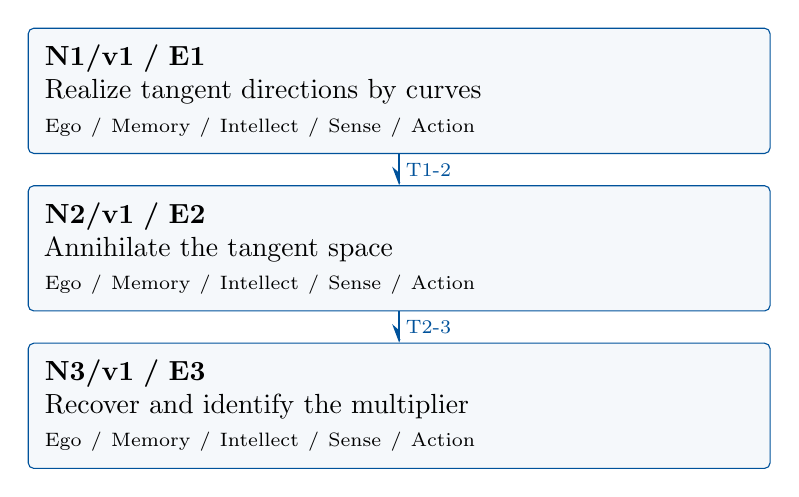
\begin{tikzpicture}[>=Stealth,x=1cm,y=1cm]

\node[mmnode,text width=9cm,minimum height=1.25cm] (N1) at (0,0.0) {\textbf{N1/v1 / E1}\\Realize tangent directions by curves\\{\scriptsize Ego / Memory / Intellect / Sense / Action}};

\node[mmnode,text width=9cm,minimum height=1.25cm] (N2) at (0,-2.0) {\textbf{N2/v1 / E2}\\Annihilate the tangent space\\{\scriptsize Ego / Memory / Intellect / Sense / Action}};

\node[mmnode,text width=9cm,minimum height=1.25cm] (N3) at (0,-4.0) {\textbf{N3/v1 / E3}\\Recover and identify the multiplier\\{\scriptsize Ego / Memory / Intellect / Sense / Action}};

\draw[mmproof] (N1.south) -- node[mmnote,right] {T1-2} (N2.north);

\draw[mmproof] (N2.south) -- node[mmnote,right] {T2-3} (N3.north);

\end{tikzpicture}\end{center}

Each box is one mathematical agent containing all five faculties. Blue
arrows carry the versioned exports listed below. The layout gives a
reading order; only drawn arrows assert dependencies. Diagnostic repair
is separate from the proof DAG.

\subsection{Versioned evidence-transfer ledger}

\begingroup\small\linespread{1.05}\selectfont

\Needspace{5\baselineskip}\field{T1-2: N1/E1/v1 to N2}{For every \(v\in\ker A\) there is a \(C^1\) feasible curve \(\gamma\)
through \(x_*\) with \(\gamma'(0)=v\).}

\field{Receiving activity}{N2.1}

\field{Compatibility}{E1/v1 and local constrained extremality. Check: Both signs of the curve
parameter are available locally, allowing a zero derivative rather than
a one-sided inequality.}

\Needspace{5\baselineskip}\field{T2-3: N2/E2/v1 to N3}{\(\nabla f(x_*)\in(\ker A)^\perp\).}

\field{Receiving activity}{N3.1}

\field{Compatibility}{E2/v1 and rank \(A=m\). Check: Uniqueness of the multiplier uses
injectivity of \(A^T\), not uniqueness of the constrained optimum.}

\endgroup

\clearpage\section{Agent roles and five-faculty activities}\begingroup\small\linespread{1.05}\selectfont\setlist{itemsep=1pt,topsep=2pt}

\subsection{N1/v1: Realize tangent directions by curves}

\field{Object and role}{Use the implicit graph to convert a linearized feasible direction into a
genuinely feasible curve. \textbf{Local obligation:} For every
\(v\in\ker A\) there is a \(C^1\) feasible curve \(\gamma\) through
\(x_*\) with \(\gamma'(0)=v\).}

\field{Inputs}{\(A=Dh(x_*)\) of rank \(m\), and \(v\in\ker A\).}

\mmfaculty{E}{Ego}{Publish E1/v1 only after establishing this obligation: For every
\(v\in\ker A\) there is a \(C^1\) feasible curve \(\gamma\) through
\(x_*\) with \(\gamma'(0)=v\).}

\mmfaculty{M}{Memory}{\(A=Dh(x_*)\) of rank \(m\), and \(v\in\ker A\). Retain the stated
assumptions and import versions.}

\mmfaculty{I}{Intellect}{Use the implicit graph to convert a linearized feasible direction into a
genuinely feasible curve.}

\mmfaculty{S}{Sense}{The invertible coordinate block is guaranteed by rank \(m\); without it,
the kernel may overestimate actual tangent directions.}

\mmfaculty{A}{Action}{Carry out activities N1.1--N1.2 below, retaining each calculation and
construction as evidence.}

\smallskip\noindent\textbf{Numbered mathematical activities}

\begin{enumerate}[label=N1.\arabic*,leftmargin=3.4em]

\item After permuting coordinates write \(x=(y,z)\) with \(y\in\mathbb R^m\)
and \(D_yh(x_*)\) invertible. The implicit function theorem writes
nearby feasible points as \((\phi(z),z)\), with \(\phi(z_*)=y_*\).
Differentiating \(h(\phi(z),z)=0\) gives
\(D\phi(z_*)=-(D_yh)^{-1}D_zh\), all derivatives evaluated at \(x_*\).

\item Write \(v=(v_y,v_z)\). The equation \(Av=0\) says \(v_y=D\phi(z_*)v_z\).
Hence \(\gamma(t)=(\phi(z_*+tv_z),z_*+tv_z)\) is feasible for small
positive and negative \(t\), passes through \(x_*\), and has derivative
\(v\).

\end{enumerate}

\field{Export E1/v1}{For every \(v\in\ker A\) there is a \(C^1\) feasible curve \(\gamma\)
through \(x_*\) with \(\gamma'(0)=v\).}

\field{Acceptance gate}{The invertible coordinate block is guaranteed by rank \(m\); without it,
the kernel may overestimate actual tangent directions.}

\field{Targeted repair}{If a kernel vector is declared tangent without a feasible curve,
construct it through the implicit graph and check the full-rank
hypothesis. Withhold this export and recheck its descendants after a
versioned correction.}

\clearpage

\subsection{N2/v1: Annihilate the tangent space}

\field{Object and role}{Differentiate the objective along each two-sided feasible curve.
\textbf{Local obligation:} \(\nabla f(x_*)\in(\ker A)^\perp\).}

\field{Inputs}{E1/v1 and local constrained extremality. Incoming proof exports: E1/v1
at N2.1.}

\mmfaculty{E}{Ego}{Publish E2/v1 only after establishing this obligation:
\(\nabla f(x_*)\in(\ker A)^\perp\).}

\mmfaculty{M}{Memory}{E1/v1 and local constrained extremality. Incoming proof exports: E1/v1
at N2.1. Retain the stated assumptions and import versions.}

\mmfaculty{I}{Intellect}{Differentiate the objective along each two-sided feasible curve.}

\mmfaculty{S}{Sense}{Both signs of the curve parameter are available locally, allowing a zero
derivative rather than a one-sided inequality.}

\mmfaculty{A}{Action}{Carry out activities N2.1--N2.2 below, retaining each calculation and
construction as evidence.}

\smallskip\noindent\textbf{Numbered mathematical activities}

\begin{enumerate}[label=N2.\arabic*,leftmargin=3.4em]

\item For each \(v\in\ker A\), choose the curve from E1. The scalar \(C^1\)
function \(t\mapsto f(\gamma(t))\) has a local extremum at the interior
parameter value zero. Its derivative is therefore zero.

\item The chain rule gives that derivative as
\(\langle\nabla f(x_*),v\rangle\). Since \(v\) was arbitrary in
\(\ker A\), the gradient annihilates that kernel.

\end{enumerate}

\field{Export E2/v1}{\(\nabla f(x_*)\in(\ker A)^\perp\).}

\field{Acceptance gate}{Both signs of the curve parameter are available locally, allowing a zero
derivative rather than a one-sided inequality.}

\field{Targeted repair}{If an ambient extremum is assumed instead of a constrained one, apply
stationarity only to the feasible curves already constructed. Withhold
this export and recheck its descendants after a versioned correction.}

\clearpage

\subsection{N3/v1: Recover and identify the multiplier}

\field{Object and role}{Identify the orthogonal complement of the kernel with the image of
\(A^T\). \textbf{Local obligation:} There is a unique \(\lambda\) with
\(\nabla f(x_*)=A^T\lambda\).}

\field{Inputs}{E2/v1 and rank \(A=m\). Incoming proof exports: E2/v1 at N3.1.}

\mmfaculty{E}{Ego}{Publish E3/v1 only after establishing this obligation: There is a unique
\(\lambda\) with \(\nabla f(x_*)=A^T\lambda\).}

\mmfaculty{M}{Memory}{E2/v1 and rank \(A=m\). Incoming proof exports: E2/v1 at N3.1. Retain
the stated assumptions and import versions.}

\mmfaculty{I}{Intellect}{Identify the orthogonal complement of the kernel with the image of
\(A^T\).}

\mmfaculty{S}{Sense}{Uniqueness of the multiplier uses injectivity of \(A^T\), not uniqueness
of the constrained optimum.}

\mmfaculty{A}{Action}{Carry out activities N3.1--N3.2 below, retaining each calculation and
construction as evidence.}

\smallskip\noindent\textbf{Numbered mathematical activities}

\begin{enumerate}[label=N3.\arabic*,leftmargin=3.4em]

\item For any \(\lambda\) and \(v\in\ker A\),
\(\langle A^T\lambda,v\rangle=\langle\lambda,Av\rangle=0\), so
\(\operatorname{im}A^T\subset(\ker A)^\perp\). The two spaces have
dimension \(m\), giving equality. E2 therefore supplies a multiplier.

\item If \(A^T\lambda=A^T\mu\), then \(A^T(\lambda-\mu)=0\). Full row rank
makes \(A^T\) injective, so \(\lambda=\mu\). No conclusion that every
multiplier solution is an extremum has been used.

\end{enumerate}

\field{Export E3/v1}{There is a unique \(\lambda\) with \(\nabla f(x_*)=A^T\lambda\).}

\field{Acceptance gate}{Uniqueness of the multiplier uses injectivity of \(A^T\), not uniqueness
of the constrained optimum.}

\field{Targeted repair}{If multiplier existence is treated as sufficient for optimality, retain
only the necessary condition and perform a separate second-order or
convexity analysis. Withhold this export and recheck its descendants
after a versioned correction.}

\endgroup\clearpage\section{Continuous mathematical proof}\label{sec:proof}

\subsection{N1 --- Realize tangent directions by
curves}\label{n1-realize-tangent-directions-by-curves}

\begin{enumerate}
\def\labelenumi{\arabic{enumi}.}
\item
  \textbf{N1.1.} After permuting coordinates write \(x=(y,z)\) with
  \(y\in\mathbb R^m\) and \(D_yh(x_*)\) invertible. The implicit
  function theorem writes nearby feasible points as \((\phi(z),z)\),
  with \(\phi(z_*)=y_*\). Differentiating \(h(\phi(z),z)=0\) gives
  \(D\phi(z_*)=-(D_yh)^{-1}D_zh\), all derivatives evaluated at \(x_*\).
\item
  \textbf{N1.2.} Write \(v=(v_y,v_z)\). The equation \(Av=0\) says
  \(v_y=D\phi(z_*)v_z\). Hence \(\gamma(t)=(\phi(z_*+tv_z),z_*+tv_z)\)
  is feasible for small positive and negative \(t\), passes through
  \(x_*\), and has derivative \(v\).
\end{enumerate}

\subsection{N2 --- Annihilate the tangent
space}\label{n2-annihilate-the-tangent-space}

\begin{enumerate}
\def\labelenumi{\arabic{enumi}.}
\item
  \textbf{N2.1.} For each \(v\in\ker A\), choose the curve from E1. The
  scalar \(C^1\) function \(t\mapsto f(\gamma(t))\) has a local extremum
  at the interior parameter value zero. Its derivative is therefore
  zero.
\item
  \textbf{N2.2.} The chain rule gives that derivative as
  \(\langle\nabla f(x_*),v\rangle\). Since \(v\) was arbitrary in
  \(\ker A\), the gradient annihilates that kernel.
\end{enumerate}

\subsection{N3 --- Recover and identify the
multiplier}\label{n3-recover-and-identify-the-multiplier}

\begin{enumerate}
\def\labelenumi{\arabic{enumi}.}
\item
  \textbf{N3.1.} For any \(\lambda\) and \(v\in\ker A\),
  \(\langle A^T\lambda,v\rangle=\langle\lambda,Av\rangle=0\), so
  \(\operatorname{im}A^T\subset(\ker A)^\perp\). The two spaces have
  dimension \(m\), giving equality. E2 therefore supplies a multiplier.
\item
  \textbf{N3.2.} If \(A^T\lambda=A^T\mu\), then \(A^T(\lambda-\mu)=0\).
  Full row rank makes \(A^T\) injective, so \(\lambda=\mu\). No
  conclusion that every multiplier solution is an extremum has been
  used.
\end{enumerate}

\hfill$\square$

\section{Worked orchestration}

Minimize \(f(x,y)=x^2+y^2\) subject to \(h(x,y)=x+y-1=0\). The gradient
equation is \((2x,2y)=\lambda(1,1)\), hence \(x=y=1/2\) and
\(\lambda=1\). Substituting \(y=1-x\) gives \(f=2(x-1/2)^2+1/2\),
separately verifying that this stationary point is the global minimum.

\subsection{Boundary and hypothesis audit}

If rank fails, take \(f(x,y)=x\) and \(h(x,y)=x^2+y^2\). The feasible
set is the single point \((0,0)\), which is both a constrained minimum
and maximum, but \(\nabla f=(1,0)\) while \(Dh=(0,0)\), so no multiplier
exists. Sufficiency also fails: for \(f(x,y)=x^3\) subject to \(y=0\),
the origin satisfies the multiplier equation but is not an extremum.

\section{Illustrative failure and repair}

The following is an authored diagnostic scenario. Changed assumptions
define a new contract; they do not retroactively prove the original
statement.

\subsection{Rejected argument, diagnosis, and correction}
\textbf{Rejected N1 inference:} every vector in \(\ker Dh\) is the
velocity of a feasible curve, without a rank condition. The single-point
constraint has \(\ker Dh=\mathbb R^2\) at zero but only zero feasible
velocities. \textbf{Repair:} invoke full rank and the implicit graph
exactly as N1 does. The original theorem is preserved; the rank-free
extension is rejected. Recheck tangent annihilation and multiplier
existence.

\subsection{Publication and reuse}
The corrected export retains its explicit assumptions. A hypothetical
revision receives a new version, and each consuming activity is
rechecked; this scenario is not a recorded runtime event. \textbf{Next
direction:} Develop second-order conditions on the tangent space,
explicitly separating necessary and sufficient tests.

\par\medskip\begingroup\small\linespread{1.0}\selectfont\noindent\textbf{Provenance.} This authored proof is complete relative to its declared imports. Reuse
each export with its assumptions, proof, and version. The original
Markdown remains available for comparison.
\par\endgroup

\par\smallskip\begingroup\small\linespread{1.0}\selectfont\noindent\textbf{Further reading.} \href{https://web.stanford.edu/~boyd/cvxbook/}{Boyd and Vandenberghe,
Convex Optimization} for convexity, optimality, and descent;
\href{https://www.math.umd.edu/~mariakc/Spring2020Class.html}{University
of Maryland, Scientific Computing I} for the numerical-analysis setting.
The estimates used here are derived explicitly in §4.\par\endgroup

\end{document}
